\documentclass[17pt]{article}

% if you need to pass options to natbib, use, e.g.:
%     \PassOptionsToPackage{numbers, compress}{natbib}
% before loading neurips_2019

% ready for submission
% \usepackage{neurips_2019}

% to compile a preprint version, e.g., for submission to arXiv, add add the
% [preprint] option:
    % \usepackage[preprint]{neurips_2019}

% to compile a camera-ready version, add the [final] option, e.g.:
\usepackage[final]{neurips}
\linespread{1.6} % عدد بین 1.2 تا 2 بسته به نیاز


% to avoid loading the natbib package, add option nonatbib:
    % \usepackage[nonatbib]{neurips_2019}

\usepackage[utf8]{inputenc} % allow utf-8 input
\usepackage[T1]{fontenc}    % use 8-bit T1 fonts
\usepackage{hyperref}       % hyperlinks
\usepackage{url}            % simple URL typesetting
\usepackage{booktabs}       % professional-quality tables
\usepackage{amsfonts}       % blackboard math symbols
\usepackage{nicefrac}       % compact symbols for 1/2, etc.
\usepackage{microtype}      % microtypography
\usepackage{graphicx}
\usepackage{xepersian}
\settextfont{XB Yas.ttf}
\usepackage{fontspec}
\usepackage{fancyhdr}
\usepackage{amsmath}
\usepackage{array}
\usepackage{pgfplots} % For bar charts

\usepackage{algorithm}      % For algorithm float
\usepackage[noend]{algpseudocode}  % For pseudocode formatting
\usepackage{amssymb}  



\usepackage{pgfplots}
\pagestyle{fancy}
\fancyhf{}
\fancyhead[LE,RO]{\thepage}
\fancyhead[RE]{\leftmark}
\fancyhead[LO]{\rightmark}
\newcommand{\code}[1]{\texttt{\color{codeblue}#1}}




\usepackage{listings}
\usepackage{xcolor}

\definecolor{codebg}{rgb}{0.97,0.97,0.97}
\definecolor{codegray}{gray}{0.4}
\definecolor{codeblue}{rgb}{0.2,0.3,0.8}




\definecolor{codegreen}{rgb}{0,0.6,0}      % comments
\definecolor{codegray}{rgb}{0.5,0.5,0.5}   % line numbers
\definecolor{codepurple}{rgb}{0.58,0,0.82} % strings
\definecolor{backcolour}{rgb}{0.95,0.95,0.92} % background
\definecolor{blue}{rgb}{0,0,0.8}           % opcodes
\definecolor{magenta}{rgb}{0.7,0,0.7}      % directives/punctuation

\lstdefinestyle{cppstyle}{
  backgroundcolor=\color{codebg},
  commentstyle=\color{codegray}\itshape,
  keywordstyle=\color{codeblue}\bfseries,
  numberstyle=\tiny\color{gray},
  stringstyle=\color{red!60!brown},
  basicstyle=\ttfamily\small,
  breaklines=true,
  numbers=left,
  numbersep=8pt,
  tabsize=4,
  language=C++
}

\lstset{style=cppstyle}


\title{پیاده سازی Policy Replacement های مختلف و بررسی و مقایسهٔ کارایی آن ها به وسیلهٔ شبیه ساز ChampSim}




% The \author macro works with any number of authors. There are two commands
% used to separate the names and addresses of multiple authors: \And and \AND.
%
% Using \And between authors leaves it to LaTeX to determine where to break the
% lines. Using \AND forces a line break at that point. So, if LaTeX puts 3 of 4
% authors names on the first line, and the last on the second line, try using
% \AND instead of \And before the third author name.

\author{%
  \begin{tabular}{@{}c@{}}
    نویسنده‌\\
    مهدیار صلواتی\\
    کد دانشجویی: 402243080\\
    \texttt{ma.salavati@mail.sbu.ac.ir}
  \end{tabular}%
}



% create title (includes both anonymized and non-anonymized versions)
% \providecommand{\@makepertitle}{}
% \newcommand{\makepertitle}{%
%   \vbox{%
%     \hsize\textwidth
%     \linewidth\hsize
%     \vskip 0.1in
%     \toptitlebar
%     \centering
%     {\LARGE\bf \@title\par}
%     \bottomtitlebar
%       \def\And{%
%         \end{tabular}\hfil\linebreak[0]\hfil%
%         \begin{tabular}[t]{c}\bf\rule{\z@}{24\p@}\ignorespaces%
%       }
%       \def\AND{%
%         \end{tabular}\hfil\linebreak[4]\hfil%
%         \begin{tabular}[t]{c}\bf\rule{\z@}{24\p@}\ignorespaces%
%       }
%       \begin{tabular}[t]{c}\bf\rule{\z@}{24\p@}\@author\end{tabular}%
%     \vskip 0.3in \@minus 0.1in
%   }
% }

\begin{document}


\begin{minipage}{0.1\textwidth}% adapt widths of minipages to your needs

\end{minipage}%
\hfill%
\begin{minipage}{0.9\textwidth}\raggedleft
 پروژهٔ نهایی درس معماری کامپیوتر\\
استاد: دکتر چشمی خانی\\
\end{minipage}
% \end{}


\makepertitle


\begin{abstract}
در این پروژه قصد داریم سیاست های جانشینی LRU، LFU، MRU و FIFO را با استفاده از زبان C پیاده کرده و هر یک را با 60 میلیون instruction warmup و 40 میلیون instruction simulate شبیه سازی کرده و در نهایت پارامتر های Rate Miss - Rate Hit - IPC Cumulative را تفسیر و مقایسه کنیم.
در تمامی تست ها از trace زیر استفاده شده است:
bzip2\_183B.trace.xz
\end{abstract}


\section{LRU}
\subsection{پیاده سازی الگوریتم}
این سیاست جایگزینی بر اساس سن هر کدام از بلاک های کش کار می کند. یعنی وقتی کش پر شود و درخواست بلاک جدیدی دریافت شود، این سیاست بلاکی را اخراج می کند که از همه پیر تر یا به اصطلاح Used Recently Least است.
منطقی است که در زمان hit شدن هر بلاک، آن بلاک به عنوان MRU شناخته شده و باقی بلاک ها پیر تر می شوند.

در اینجا ما کد C را بر اساس شماره clock که در آن قرار داریم پیاده می کنیم. یعنی یک آرایه به نام last\_used\_cycles به طول تعداد بلاک ها allocate کرده و به عنوان مقادیر اولیه صفر در درایه های آن وارد می کنیم.


همچنین سایز این آرایه که همان تعداد بلاک ها است را می توان این گونه محاسبه کرد که کش دارای set x است و هر ست دارای way y است. در نتیجه تعداد کل بلاک ها از حاصل ضرب x و y محاسبه می شود و در نهایت Constructor ما به این شکل در می آید:

\begin{LTR}
\begin{lstlisting}
myLRU::myLRU(...) {
    cycle_array_size = (size_t)(sets * ways);
    last_used_cycles = new uint64_t[cycle_array_size];
    for (size_t i = 0; i < cycle_array_size; i++) {
        last_used_cycles[i] = 0;
    }
}
\end{lstlisting}
\end{LTR}

با هر بار پر شدن یکی از way ها تابع fill cache replacement فراخوانی می شود. در این جا با توجه به توضیحاتی که دادیم، ابتدا شماره cycle که در آن قرار داریم را به عنوان درایهٔ آن way مورد نطر قرار داده و در نهایت cycle را increment می کنیم:

\begin{LTR}
\begin{lstlisting}
 void myLRU::replacement_cache_fill(...)
{
    last_used_cycles[(size_t)(set * NUM_WAY + way)] = cycle++;
}
\end{lstlisting}
\end{LTR}

شایان ذکر است که تابع بالا وقتی فراخوانی می شود که بلاک مورد نظر خالی بوده و یا محتوای جایگزین شده در آن miss شده بود و تابع state replacement update زمانی رخ می دهد که شاهد hit باشیم.

حال که معانی اعداد داخل آرایه را بررسی کردیم به راحتی می توانیم تابع find\_victim را بررسی کنیم. این تابع بلاکی را اخراج می کند که last\_used\_cycles کمتری داشته باشد چرا که قدیمی تر است:

\begin{LTR}
\begin{lstlisting}
long myLRU::find_victim(...)
{
    long set_offset = set * NUM_WAY;
    long victim_way = 0;
    uint64_t min_cycle = last_used_cycles[set_offset];

    for (long i = 1; i < NUM_WAY; i++) {
        if (last_used_cycles[set_offset + i] < min_cycle) {
            min_cycle = last_used_cycles[set_offset + i];
            victim_way = i;
        }
    }

    assert(victim_way >= 0);
    assert(victim_way < NUM_WAY);
    return victim_way;
}
\end{lstlisting}
\end{LTR}

\subsection{شبیه سازی}
در این شبیه سازی و شبیه سازی های آتی پس از آپدیت کردن محتوای فایل champsim\_config.jsonاز دستور های زیر استفاده می کنیم:
\begin{LTR}
\begin{lstlisting}
./config.sh champsim_config.json
make
bin/champsim --warmup-instructions 60000000 --simulation-instructions 40000000 /Users/mahdiyarsalavati/Downloads/bzip2_183B.trace.xz
\end{lstlisting}
\end{LTR}

نتایج خام شبیه سازی:

\begin{LTR}
\begin{lstlisting}[basicstyle=\tiny\ttfamily]
mahdiyarsalavati@Mahdiyars-MacBook-Air ChampSimLocal % bin/champsim --warmup-instructions 60000000 --simulation-instructions 40000000 /Users/mahdiyarsalavati/Downloads/bzip2_183B.trace.xz
[VMEM] WARNING: physical memory size is smaller than virtual memory size.

*** ChampSim Multicore Out-of-Order Simulator ***
Warmup Instructions: 60000000
Simulation Instructions: 40000000
Number of CPUs: 1
Page size: 4096

Off-chip DRAM Size: 16 GiB Channels: 1 Width: 64-bit Data Rate: 3205 MT/s
Heartbeat CPU 0 instructions: 10000003 cycles: 2573517 heartbeat IPC: 3.886 cumulative IPC: 3.886 (Simulation time: 00 hr 00 min 18 sec)
Heartbeat CPU 0 instructions: 20000005 cycles: 5086294 heartbeat IPC: 3.98 cumulative IPC: 3.932 (Simulation time: 00 hr 00 min 36 sec)
Heartbeat CPU 0 instructions: 30000007 cycles: 7597883 heartbeat IPC: 3.982 cumulative IPC: 3.948 (Simulation time: 00 hr 00 min 54 sec)
Heartbeat CPU 0 instructions: 40000008 cycles: 10110284 heartbeat IPC: 3.98 cumulative IPC: 3.956 (Simulation time: 00 hr 01 min 12 sec)
Heartbeat CPU 0 instructions: 50000008 cycles: 12624634 heartbeat IPC: 3.977 cumulative IPC: 3.961 (Simulation time: 00 hr 01 min 30 sec)
Warmup finished CPU 0 instructions: 60000000 cycles: 15140864 cumulative IPC: 3.963 (Simulation time: 00 hr 01 min 48 sec)
Warmup complete CPU 0 instructions: 60000000 cycles: 15140864 cumulative IPC: 3.963 (Simulation time: 00 hr 01 min 48 sec)
Heartbeat CPU 0 instructions: 60000008 cycles: 15140866 heartbeat IPC: 3.974 cumulative IPC: 4 (Simulation time: 00 hr 01 min 48 sec)
Heartbeat CPU 0 instructions: 70000010 cycles: 22365020 heartbeat IPC: 1.384 cumulative IPC: 1.384 (Simulation time: 00 hr 02 min 15 sec)
Heartbeat CPU 0 instructions: 80000010 cycles: 29110017 heartbeat IPC: 1.483 cumulative IPC: 1.432 (Simulation time: 00 hr 02 min 42 sec)
Heartbeat CPU 0 instructions: 90000010 cycles: 36163222 heartbeat IPC: 1.418 cumulative IPC: 1.427 (Simulation time: 00 hr 03 min 11 sec)
Simulation finished CPU 0 instructions: 40000001 cycles: 28788163 cumulative IPC: 1.389 (Simulation time: 00 hr 03 min 40 sec)
Simulation complete CPU 0 instructions: 40000001 cycles: 28788163 cumulative IPC: 1.389 (Simulation time: 00 hr 03 min 40 sec)

ChampSim completed all CPUs

=== Simulation ===
CPU 0 runs /Users/mahdiyarsalavati/Downloads/bzip2_183B.trace.xz

Region of Interest Statistics

CPU 0 cumulative IPC: 1.389 instructions: 40000001 cycles: 28788163
CPU 0 Branch Prediction Accuracy: 88.8% MPKI: 19.68 Average ROB Occupancy at Mispredict: 21.49
Branch type MPKI
BRANCH_DIRECT_JUMP: 0.0478
BRANCH_INDIRECT: 0
BRANCH_CONDITIONAL: 19.63
BRANCH_DIRECT_CALL: 0
BRANCH_INDIRECT_CALL: 0
BRANCH_RETURN: 0

cpu0->cpu0_STLB TOTAL        ACCESS:     214404 HIT:     214253 MISS:        151 MSHR_MERGE:          0
cpu0->cpu0_STLB LOAD         ACCESS:     214404 HIT:     214253 MISS:        151 MSHR_MERGE:          0
cpu0->cpu0_STLB RFO          ACCESS:          0 HIT:          0 MISS:          0 MSHR_MERGE:          0
cpu0->cpu0_STLB PREFETCH     ACCESS:          0 HIT:          0 MISS:          0 MSHR_MERGE:          0
cpu0->cpu0_STLB WRITE        ACCESS:          0 HIT:          0 MISS:          0 MSHR_MERGE:          0
cpu0->cpu0_STLB TRANSLATION  ACCESS:          0 HIT:          0 MISS:          0 MSHR_MERGE:          0
cpu0->cpu0_STLB PREFETCH REQUESTED:          0 ISSUED:          0 USEFUL:          0 USELESS:          0
cpu0->cpu0_STLB AVERAGE MISS LATENCY: 792 cycles
cpu0->cpu0_L2C TOTAL        ACCESS:     816970 HIT:     536435 MISS:     280535 MSHR_MERGE:          0
cpu0->cpu0_L2C LOAD         ACCESS:     480429 HIT:     315435 MISS:     164994 MSHR_MERGE:          0
cpu0->cpu0_L2C RFO          ACCESS:     157239 HIT:      41980 MISS:     115259 MSHR_MERGE:          0
cpu0->cpu0_L2C PREFETCH     ACCESS:          0 HIT:          0 MISS:          0 MSHR_MERGE:          0
cpu0->cpu0_L2C WRITE        ACCESS:     179018 HIT:     178988 MISS:         30 MSHR_MERGE:          0
cpu0->cpu0_L2C TRANSLATION  ACCESS:        284 HIT:         32 MISS:        252 MSHR_MERGE:          0
cpu0->cpu0_L2C PREFETCH REQUESTED:          0 ISSUED:          0 USEFUL:          0 USELESS:          0
cpu0->cpu0_L2C AVERAGE MISS LATENCY: 89.21 cycles
cpu0->cpu0_L1I TOTAL        ACCESS:    1200398 HIT:    1200398 MISS:          0 MSHR_MERGE:          0
cpu0->cpu0_L1I LOAD         ACCESS:    1200398 HIT:    1200398 MISS:          0 MSHR_MERGE:          0
cpu0->cpu0_L1I RFO          ACCESS:          0 HIT:          0 MISS:          0 MSHR_MERGE:          0
cpu0->cpu0_L1I PREFETCH     ACCESS:          0 HIT:          0 MISS:          0 MSHR_MERGE:          0
cpu0->cpu0_L1I WRITE        ACCESS:          0 HIT:          0 MISS:          0 MSHR_MERGE:          0
cpu0->cpu0_L1I TRANSLATION  ACCESS:          0 HIT:          0 MISS:          0 MSHR_MERGE:          0
cpu0->cpu0_L1I PREFETCH REQUESTED:          0 ISSUED:          0 USEFUL:          0 USELESS:          0
cpu0->cpu0_L1I AVERAGE MISS LATENCY: - cycles
cpu0->cpu0_L1D TOTAL        ACCESS:   11538774 HIT:   10699096 MISS:     839678 MSHR_MERGE:     201724
cpu0->cpu0_L1D LOAD         ACCESS:    8591790 HIT:    7963728 MISS:     628062 MSHR_MERGE:     147632
cpu0->cpu0_L1D RFO          ACCESS:          0 HIT:          0 MISS:          0 MSHR_MERGE:          0
cpu0->cpu0_L1D PREFETCH     ACCESS:          0 HIT:          0 MISS:          0 MSHR_MERGE:          0
cpu0->cpu0_L1D WRITE        ACCESS:    2946682 HIT:    2735358 MISS:     211324 MSHR_MERGE:      54084
cpu0->cpu0_L1D TRANSLATION  ACCESS:        302 HIT:         10 MISS:        292 MSHR_MERGE:          8
cpu0->cpu0_L1D PREFETCH REQUESTED:          0 ISSUED:          0 USEFUL:          0 USELESS:          0
cpu0->cpu0_L1D AVERAGE MISS LATENCY: 47.97 cycles
cpu0->cpu0_ITLB TOTAL        ACCESS:     960937 HIT:     960937 MISS:          0 MSHR_MERGE:          0
cpu0->cpu0_ITLB LOAD         ACCESS:     960937 HIT:     960937 MISS:          0 MSHR_MERGE:          0
cpu0->cpu0_ITLB RFO          ACCESS:          0 HIT:          0 MISS:          0 MSHR_MERGE:          0
cpu0->cpu0_ITLB PREFETCH     ACCESS:          0 HIT:          0 MISS:          0 MSHR_MERGE:          0
cpu0->cpu0_ITLB WRITE        ACCESS:          0 HIT:          0 MISS:          0 MSHR_MERGE:          0
cpu0->cpu0_ITLB TRANSLATION  ACCESS:          0 HIT:          0 MISS:          0 MSHR_MERGE:          0
cpu0->cpu0_ITLB PREFETCH REQUESTED:          0 ISSUED:          0 USEFUL:          0 USELESS:          0
cpu0->cpu0_ITLB AVERAGE MISS LATENCY: - cycles
cpu0->cpu0_DTLB TOTAL        ACCESS:   10984452 HIT:   10729968 MISS:     254484 MSHR_MERGE:      40081
cpu0->cpu0_DTLB LOAD         ACCESS:   10984452 HIT:   10729968 MISS:     254484 MSHR_MERGE:      40081
cpu0->cpu0_DTLB RFO          ACCESS:          0 HIT:          0 MISS:          0 MSHR_MERGE:          0
cpu0->cpu0_DTLB PREFETCH     ACCESS:          0 HIT:          0 MISS:          0 MSHR_MERGE:          0
cpu0->cpu0_DTLB WRITE        ACCESS:          0 HIT:          0 MISS:          0 MSHR_MERGE:          0
cpu0->cpu0_DTLB TRANSLATION  ACCESS:          0 HIT:          0 MISS:          0 MSHR_MERGE:          0
cpu0->cpu0_DTLB PREFETCH REQUESTED:          0 ISSUED:          0 USEFUL:          0 USELESS:          0
cpu0->cpu0_DTLB AVERAGE MISS LATENCY: 5.559 cycles
cpu0->LLC TOTAL        ACCESS:     409061 HIT:     345389 MISS:      63672 MSHR_MERGE:          0
cpu0->LLC LOAD         ACCESS:     164994 HIT:     135503 MISS:      29491 MSHR_MERGE:          0
cpu0->LLC RFO          ACCESS:     115259 HIT:      81332 MISS:      33927 MSHR_MERGE:          0
cpu0->LLC PREFETCH     ACCESS:          0 HIT:          0 MISS:          0 MSHR_MERGE:          0
cpu0->LLC WRITE        ACCESS:     128556 HIT:     128553 MISS:          3 MSHR_MERGE:          0
cpu0->LLC TRANSLATION  ACCESS:        252 HIT:          1 MISS:        251 MSHR_MERGE:          0
cpu0->LLC PREFETCH REQUESTED:          0 ISSUED:          0 USEFUL:          0 USELESS:          0
cpu0->LLC AVERAGE MISS LATENCY: 325.7 cycles

DRAM Statistics

Channel 0 RQ ROW_BUFFER_HIT:       2779
  ROW_BUFFER_MISS:      60613
  AVG DBUS CONGESTED CYCLE: 12.16
Channel 0 WQ ROW_BUFFER_HIT:       9245
  ROW_BUFFER_MISS:      37224
  FULL:          0
Channel 0 REFRESHES ISSUED:       2399
\end{lstlisting}
\end{LTR}

حال با توجه به دو فرمول زیر پارامتر های خواسته شده را بدست می آوریم:


\begin{center}
\[
\text{\lr{Miss Rate}} = \frac{\text{\lr{\# of misses}}}{\text{\lr{\# of total accesses}}} \times 100 = \frac{63672}{409061} \times 100 = \boxed{15.57\%}
\]

\vspace{0.2cm} % Vertical spacing between equations

\[
\text{\lr{Hit Rate}} = \frac{\text{\lr{\# of hits}}}{\text{\lr{\lr{\# of total accesses}}}} \times 100 = \frac{345389}{409061} \times 100 = \boxed{84.43\%}
\]

\vspace{0.2cm} % Larger spacing before the last equation

\[
\text{\lr{Cumulative IPC}} = \boxed{1.389}
\]
\end{center}

توضیحات مربوط به نرخ تصادم و نرخ miss به صورت فرمول ریاضی داده شد. پارامتر IPC Cumulative نشان دهندهٔ تعداد Instruction هایی است که در یک کلاک می توانند انجام شوند. 
کلمهٔ Cumulative به این معناست که عدد نهایی تجمیعی از IPC هایی است که در طول شبیه سازی با آنها مواجه بودیم. برای مثال شبیه سازی با IPC Heartbeat برابر ۹۷۴.۳ شروع به کار کرد اما با پیشرفت در شبیه سازی این مقدار کمتر شد.

به طور کلی می توان گفت این سیاست عملکرد مناسبی داشته و شاهد Hit Rate بالایی هستیم و مقدار Clock Per Instrucion نیز عدد مطلوبی به نظر می رسد. در نهایت با مقایسهٔ این چهار روش، به دید بهتری از این اعداد خواهیم رسید.

\section{LFU}
\subsection{پیاده سازی الگوریتم}
این سیاست جایگزینی بر اساس فراوانی دسترسی ها به بلاک های مختلف عمل می کند. بر این اساس که دو آرایه نگه می داریم که هر دو به تعداد بلاک های کش هستند. آرایهٔ اولی مشابه LRU برای هر بلاک، آخرین کلاکی را نگه می دارد که به آن بلاک دسترسی داشته ایم. اسم این آرایه  مانند گذشته last\_used\_cycles است. اما آرایهٔ دوم همان چیزی است که این سیاست را از LRU متمایز می کند. این آرایه که از اسمش frequency\_counters پیداست قرار است تعداد دفعاتی را نگه دارد که هر یک از بلاک های کش فراخوانی شده اند.

در نهایت در زمان پر شدن کش، برای اخراج قربانی به این شکل عمل می کند که ابتدا بلاکی(هایی) را پیدا می کند که frequency\_counters آن ها مینیمم است. در نتیجه کمتر فراخوانی شده اند و آنها نامزد اول اخراج هستند. سپس پس از یافت آنها، آن بلاکی را اخراج می کند که از همه قدیمی تر است (یعنی آن که last\_used\_cycles کمتری دارد).

پس با توجه به توضیحات داده شده، آرایه ها در صورتی که کش خالی باشد این گونه پر می شوند:

\begin{LTR}
\begin{lstlisting}
void myLFU::replacement_cache_fill(...)
{
    size_t block_index = (size_t)(set * NUM_WAY + way);
    frequency_counters[block_index] = 1;
    last_used_cycles[block_index] = cycle++;
}
\end{lstlisting}
\end{LTR}

و در صورتی که شاهد hit باشیم این گونه محتوای آرایه ها تغییر می کند:
\begin{LTR}
\begin{lstlisting}
void myLFU::update_replacement_state(...)
{
    if (hit && access_type{type} != access_type::WRITE) {
        size_t block_index = (size_t)(set * NUM_WAY + way);
        frequency_counters[block_index]++;
        last_used_cycles[block_index] = cycle++;
    }
}
\end{lstlisting}
\end{LTR}

حال بر اساس منطق توضیح داده شده، در تابع find\_victim بلاکی که کمترین frequency و سپس کمترین سن را دارد اخراج می شود:
\begin{LTR}
\begin{lstlisting}
long myLFU::find_victim(...)
{
    long set_offset = set * NUM_WAY;

    uint64_t min_freq = frequency_counters[set_offset];
    for (long i = 1; i < NUM_WAY; i++) {
        if (frequency_counters[set_offset + i] < min_freq) {
            min_freq = frequency_counters[set_offset + i];
        }
    }

    long victim_way = -1;
    uint64_t min_cycle = std::numeric_limits<uint64_t>::max();
    for (long i = 0; i < NUM_WAY; i++) {
        if (frequency_counters[set_offset + i] == min_freq) {
            if (last_used_cycles[set_offset + i] < min_cycle) {
                min_cycle = last_used_cycles[set_offset + i];
                victim_way = i;
            }
        }
    }

    assert(victim_way != -1);
    return victim_way;
}


\end{lstlisting}
\end{LTR}


\subsection{شبیه سازی}
نتایج خام شبیه سازی:

\begin{LTR}
\begin{lstlisting}[basicstyle=\tiny\ttfamily]
	mahdiyarsalavati@Mahdiyars-MacBook-Air ChampSimLocal % bin/champsim --warmup-instructions 60000000 --simulation-instructions 40000000 /Users/mahdiyarsalavati/Downloads/bzip2_183B.trace.xz
[VMEM] WARNING: physical memory size is smaller than virtual memory size.

*** ChampSim Multicore Out-of-Order Simulator ***
Warmup Instructions: 60000000
Simulation Instructions: 40000000
Number of CPUs: 1
Page size: 4096

Off-chip DRAM Size: 16 GiB Channels: 1 Width: 64-bit Data Rate: 3205 MT/s
Heartbeat CPU 0 instructions: 10000003 cycles: 2573507 heartbeat IPC: 3.886 cumulative IPC: 3.886 (Simulation time: 00 hr 00 min 18 sec)
Heartbeat CPU 0 instructions: 20000005 cycles: 5086286 heartbeat IPC: 3.98 cumulative IPC: 3.932 (Simulation time: 00 hr 00 min 36 sec)
Heartbeat CPU 0 instructions: 30000007 cycles: 7597843 heartbeat IPC: 3.982 cumulative IPC: 3.948 (Simulation time: 00 hr 00 min 54 sec)
Heartbeat CPU 0 instructions: 40000008 cycles: 10110248 heartbeat IPC: 3.98 cumulative IPC: 3.956 (Simulation time: 00 hr 01 min 12 sec)
Heartbeat CPU 0 instructions: 50000008 cycles: 12624617 heartbeat IPC: 3.977 cumulative IPC: 3.961 (Simulation time: 00 hr 01 min 30 sec)
Warmup finished CPU 0 instructions: 60000000 cycles: 15140856 cumulative IPC: 3.963 (Simulation time: 00 hr 01 min 47 sec)
Warmup complete CPU 0 instructions: 60000000 cycles: 15140856 cumulative IPC: 3.963 (Simulation time: 00 hr 01 min 47 sec)
Heartbeat CPU 0 instructions: 60000008 cycles: 15140858 heartbeat IPC: 3.974 cumulative IPC: 4 (Simulation time: 00 hr 01 min 47 sec)
Heartbeat CPU 0 instructions: 70000010 cycles: 22539981 heartbeat IPC: 1.352 cumulative IPC: 1.352 (Simulation time: 00 hr 02 min 16 sec)
Heartbeat CPU 0 instructions: 80000010 cycles: 29384749 heartbeat IPC: 1.461 cumulative IPC: 1.404 (Simulation time: 00 hr 02 min 43 sec)
Heartbeat CPU 0 instructions: 90000010 cycles: 36367405 heartbeat IPC: 1.432 cumulative IPC: 1.413 (Simulation time: 00 hr 03 min 11 sec)
Simulation finished CPU 0 instructions: 40000001 cycles: 29309099 cumulative IPC: 1.365 (Simulation time: 00 hr 03 min 41 sec)
Simulation complete CPU 0 instructions: 40000001 cycles: 29309099 cumulative IPC: 1.365 (Simulation time: 00 hr 03 min 41 sec)

ChampSim completed all CPUs

=== Simulation ===
CPU 0 runs /Users/mahdiyarsalavati/Downloads/bzip2_183B.trace.xz

Region of Interest Statistics

CPU 0 cumulative IPC: 1.365 instructions: 40000001 cycles: 29309099
CPU 0 Branch Prediction Accuracy: 88.8% MPKI: 19.68 Average ROB Occupancy at Mispredict: 21.38
Branch type MPKI
BRANCH_DIRECT_JUMP: 0.0478
BRANCH_INDIRECT: 0
BRANCH_CONDITIONAL: 19.63
BRANCH_DIRECT_CALL: 0
BRANCH_INDIRECT_CALL: 0
BRANCH_RETURN: 0

cpu0->cpu0_STLB TOTAL        ACCESS:     214402 HIT:     214251 MISS:        151 MSHR_MERGE:          0
cpu0->cpu0_STLB LOAD         ACCESS:     214402 HIT:     214251 MISS:        151 MSHR_MERGE:          0
cpu0->cpu0_STLB RFO          ACCESS:          0 HIT:          0 MISS:          0 MSHR_MERGE:          0
cpu0->cpu0_STLB PREFETCH     ACCESS:          0 HIT:          0 MISS:          0 MSHR_MERGE:          0
cpu0->cpu0_STLB WRITE        ACCESS:          0 HIT:          0 MISS:          0 MSHR_MERGE:          0
cpu0->cpu0_STLB TRANSLATION  ACCESS:          0 HIT:          0 MISS:          0 MSHR_MERGE:          0
cpu0->cpu0_STLB PREFETCH REQUESTED:          0 ISSUED:          0 USEFUL:          0 USELESS:          0
cpu0->cpu0_STLB AVERAGE MISS LATENCY: 776.1 cycles
cpu0->cpu0_L2C TOTAL        ACCESS:     817041 HIT:     536498 MISS:     280543 MSHR_MERGE:          0
cpu0->cpu0_L2C LOAD         ACCESS:     480431 HIT:     315460 MISS:     164971 MSHR_MERGE:          0
cpu0->cpu0_L2C RFO          ACCESS:     157274 HIT:      41984 MISS:     115290 MSHR_MERGE:          0
cpu0->cpu0_L2C PREFETCH     ACCESS:          0 HIT:          0 MISS:          0 MSHR_MERGE:          0
cpu0->cpu0_L2C WRITE        ACCESS:     179052 HIT:     179022 MISS:         30 MSHR_MERGE:          0
cpu0->cpu0_L2C TRANSLATION  ACCESS:        284 HIT:         32 MISS:        252 MSHR_MERGE:          0
cpu0->cpu0_L2C PREFETCH REQUESTED:          0 ISSUED:          0 USEFUL:          0 USELESS:          0
cpu0->cpu0_L2C AVERAGE MISS LATENCY: 71.33 cycles
cpu0->cpu0_L1I TOTAL        ACCESS:    1206692 HIT:    1206692 MISS:          0 MSHR_MERGE:          0
cpu0->cpu0_L1I LOAD         ACCESS:    1206692 HIT:    1206692 MISS:          0 MSHR_MERGE:          0
cpu0->cpu0_L1I RFO          ACCESS:          0 HIT:          0 MISS:          0 MSHR_MERGE:          0
cpu0->cpu0_L1I PREFETCH     ACCESS:          0 HIT:          0 MISS:          0 MSHR_MERGE:          0
cpu0->cpu0_L1I WRITE        ACCESS:          0 HIT:          0 MISS:          0 MSHR_MERGE:          0
cpu0->cpu0_L1I TRANSLATION  ACCESS:          0 HIT:          0 MISS:          0 MSHR_MERGE:          0
cpu0->cpu0_L1I PREFETCH REQUESTED:          0 ISSUED:          0 USEFUL:          0 USELESS:          0
cpu0->cpu0_L1I AVERAGE MISS LATENCY: - cycles
cpu0->cpu0_L1D TOTAL        ACCESS:   11561545 HIT:   10716752 MISS:     844793 MSHR_MERGE:     206803
cpu0->cpu0_L1D LOAD         ACCESS:    8614517 HIT:    7971074 MISS:     643443 MSHR_MERGE:     163011
cpu0->cpu0_L1D RFO          ACCESS:          0 HIT:          0 MISS:          0 MSHR_MERGE:          0
cpu0->cpu0_L1D PREFETCH     ACCESS:          0 HIT:          0 MISS:          0 MSHR_MERGE:          0
cpu0->cpu0_L1D WRITE        ACCESS:    2946726 HIT:    2745668 MISS:     201058 MSHR_MERGE:      43784
cpu0->cpu0_L1D TRANSLATION  ACCESS:        302 HIT:         10 MISS:        292 MSHR_MERGE:          8
cpu0->cpu0_L1D PREFETCH REQUESTED:          0 ISSUED:          0 USEFUL:          0 USELESS:          0
cpu0->cpu0_L1D AVERAGE MISS LATENCY: 40.07 cycles
cpu0->cpu0_ITLB TOTAL        ACCESS:     965820 HIT:     965820 MISS:          0 MSHR_MERGE:          0
cpu0->cpu0_ITLB LOAD         ACCESS:     965820 HIT:     965820 MISS:          0 MSHR_MERGE:          0
cpu0->cpu0_ITLB RFO          ACCESS:          0 HIT:          0 MISS:          0 MSHR_MERGE:          0
cpu0->cpu0_ITLB PREFETCH     ACCESS:          0 HIT:          0 MISS:          0 MSHR_MERGE:          0
cpu0->cpu0_ITLB WRITE        ACCESS:          0 HIT:          0 MISS:          0 MSHR_MERGE:          0
cpu0->cpu0_ITLB TRANSLATION  ACCESS:          0 HIT:          0 MISS:          0 MSHR_MERGE:          0
cpu0->cpu0_ITLB PREFETCH REQUESTED:          0 ISSUED:          0 USEFUL:          0 USELESS:          0
cpu0->cpu0_ITLB AVERAGE MISS LATENCY: - cycles
cpu0->cpu0_DTLB TOTAL        ACCESS:   11006398 HIT:   10752022 MISS:     254376 MSHR_MERGE:      39975
cpu0->cpu0_DTLB LOAD         ACCESS:   11006398 HIT:   10752022 MISS:     254376 MSHR_MERGE:      39975
cpu0->cpu0_DTLB RFO          ACCESS:          0 HIT:          0 MISS:          0 MSHR_MERGE:          0
cpu0->cpu0_DTLB PREFETCH     ACCESS:          0 HIT:          0 MISS:          0 MSHR_MERGE:          0
cpu0->cpu0_DTLB WRITE        ACCESS:          0 HIT:          0 MISS:          0 MSHR_MERGE:          0
cpu0->cpu0_DTLB TRANSLATION  ACCESS:          0 HIT:          0 MISS:          0 MSHR_MERGE:          0
cpu0->cpu0_DTLB PREFETCH REQUESTED:          0 ISSUED:          0 USEFUL:          0 USELESS:          0
cpu0->cpu0_DTLB AVERAGE MISS LATENCY: 5.548 cycles
cpu0->LLC TOTAL        ACCESS:     409101 HIT:     314248 MISS:      94853 MSHR_MERGE:          0
cpu0->LLC LOAD         ACCESS:     164971 HIT:     134937 MISS:      30034 MSHR_MERGE:          0
cpu0->LLC RFO          ACCESS:     115289 HIT:      83861 MISS:      31428 MSHR_MERGE:          0
cpu0->LLC PREFETCH     ACCESS:          0 HIT:          0 MISS:          0 MSHR_MERGE:          0
cpu0->LLC WRITE        ACCESS:     128589 HIT:      95449 MISS:      33140 MSHR_MERGE:          0
cpu0->LLC TRANSLATION  ACCESS:        252 HIT:          1 MISS:        251 MSHR_MERGE:          0
cpu0->LLC PREFETCH REQUESTED:          0 ISSUED:          0 USEFUL:          0 USELESS:          0
cpu0->LLC AVERAGE MISS LATENCY: 169 cycles

DRAM Statistics

Channel 0 RQ ROW_BUFFER_HIT:       2039
  ROW_BUFFER_MISS:      59346
  AVG DBUS CONGESTED CYCLE: 13.18
Channel 0 WQ ROW_BUFFER_HIT:       9825
  ROW_BUFFER_MISS:      31625
  FULL:        130
Channel 0 REFRESHES ISSUED:       2443
\end{lstlisting}
\end{LTR}

\begin{center}
\[
\text{\lr{Miss Rate}} = \frac{\text{\lr{\# of misses}}}{\text{\lr{\# of total accesses}}} \times 100 = \frac{94853}{409101} \times 100 = \boxed{23.2\%}
\]

\vspace{0.2cm} % Vertical spacing between equations

\[
\text{\lr{Hit Rate}} = \frac{\text{\lr{\# of hits}}}{\text{\lr{\lr{\# of total accesses}}}} \times 100 = \frac{314248}{409101} \times 100 = \boxed{76.8\%}
\]

\vspace{0.2cm} % Larger spacing before the last equation

\[
\text{\lr{Cumulative IPC}} = \boxed{1.365}
\]
\end{center}

همان طور که می بینیم با آنکه شباهت زیادی هم در دو الگوریتم LRU , LFU و هم در نتایج آن وجود دارد اما می توان دید عملکرد LFU کمی بد تر از LRU بوده است. می توان ریشهٔ این رخداد را در پیچیده تر بودن سیاست LFU دانست چرا که در تابع find\_victim تقریبا به اندازهٔ دو برابر تعداد مقایسه هایی که در LRU انجام می شد، مقایسه باید انجام دهیم. البته که در برخی از ترکیب های دیگر Instruction ها سیاست LFU می تواند منجر به speed up قابل توجهی شود اما در این ترکیب از Instruction ها شاهد چنین بهبودی نبودیم.

\section{MRU}
\subsection{پیاده سازی الگوریتم}
این سیاست در پیاده سازی بسیار مشابه LRU است با این تفاوت که در تابع find\_victim آن باید ماکزیمم آرایهٔ last\_used\_cycles را به عنوان قربانی معرفی کنیم:

\begin{LTR}
\begin{lstlisting}
long myMRU::find_victim(...)
{
    long set_offset = set * NUM_WAY;
    long victim_way = 0;
    uint64_t max_cycle = last_used_cycles[set_offset];

    for (long i = 1; i < NUM_WAY; i++) {
        if (last_used_cycles[set_offset + i] > max_cycle) {
            max_cycle = last_used_cycles[set_offset + i];
            victim_way = i;
        }
    }

    assert(victim_way >= 0);
    assert(victim_way < NUM_WAY);
    return victim_way;
}
\end{lstlisting}
\end{LTR}
\subsection{شبیه سازی}
نتایج خام شبیه سازی:

\begin{LTR}
\begin{lstlisting}[basicstyle=\tiny\ttfamily]
mahdiyarsalavati@Mahdiyars-MacBook-Air ChampSimLocal % bin/champsim --warmup-instructions 60000000 --simulation-instructions 40000000 /Users/mahdiyarsalavati/Downloads/bzip2_183B.trace.xz
[VMEM] WARNING: physical memory size is smaller than virtual memory size.

*** ChampSim Multicore Out-of-Order Simulator ***
Warmup Instructions: 60000000
Simulation Instructions: 40000000
Number of CPUs: 1
Page size: 4096

Off-chip DRAM Size: 16 GiB Channels: 1 Width: 64-bit Data Rate: 3205 MT/s
Heartbeat CPU 0 instructions: 10000000 cycles: 2573519 heartbeat IPC: 3.886 cumulative IPC: 3.886 (Simulation time: 00 hr 00 min 18 sec)
Heartbeat CPU 0 instructions: 20000001 cycles: 5086305 heartbeat IPC: 3.98 cumulative IPC: 3.932 (Simulation time: 00 hr 00 min 36 sec)
Heartbeat CPU 0 instructions: 30000003 cycles: 7597899 heartbeat IPC: 3.982 cumulative IPC: 3.948 (Simulation time: 00 hr 00 min 54 sec)
Heartbeat CPU 0 instructions: 40000003 cycles: 10110316 heartbeat IPC: 3.98 cumulative IPC: 3.956 (Simulation time: 00 hr 01 min 12 sec)
Heartbeat CPU 0 instructions: 50000004 cycles: 12624668 heartbeat IPC: 3.977 cumulative IPC: 3.961 (Simulation time: 00 hr 01 min 30 sec)
Warmup finished CPU 0 instructions: 60000000 cycles: 15140901 cumulative IPC: 3.963 (Simulation time: 00 hr 01 min 48 sec)
Warmup complete CPU 0 instructions: 60000000 cycles: 15140901 cumulative IPC: 3.963 (Simulation time: 00 hr 01 min 48 sec)
Heartbeat CPU 0 instructions: 60000004 cycles: 15140902 heartbeat IPC: 3.974 cumulative IPC: 4 (Simulation time: 00 hr 01 min 48 sec)
Heartbeat CPU 0 instructions: 70000005 cycles: 24786180 heartbeat IPC: 1.037 cumulative IPC: 1.037 (Simulation time: 00 hr 02 min 25 sec)
Heartbeat CPU 0 instructions: 80000005 cycles: 33857831 heartbeat IPC: 1.102 cumulative IPC: 1.069 (Simulation time: 00 hr 03 min 00 sec)
Heartbeat CPU 0 instructions: 90000007 cycles: 43315911 heartbeat IPC: 1.057 cumulative IPC: 1.065 (Simulation time: 00 hr 03 min 38 sec)
Simulation finished CPU 0 instructions: 40000001 cycles: 39046067 cumulative IPC: 1.024 (Simulation time: 00 hr 04 min 19 sec)
Simulation complete CPU 0 instructions: 40000001 cycles: 39046067 cumulative IPC: 1.024 (Simulation time: 00 hr 04 min 19 sec)

ChampSim completed all CPUs

=== Simulation ===
CPU 0 runs /Users/mahdiyarsalavati/Downloads/bzip2_183B.trace.xz

Region of Interest Statistics

CPU 0 cumulative IPC: 1.024 instructions: 40000001 cycles: 39046067
CPU 0 Branch Prediction Accuracy: 88.8% MPKI: 19.68 Average ROB Occupancy at Mispredict: 21.95
Branch type MPKI
BRANCH_DIRECT_JUMP: 0.0478
BRANCH_INDIRECT: 0
BRANCH_CONDITIONAL: 19.63
BRANCH_DIRECT_CALL: 0
BRANCH_INDIRECT_CALL: 0
BRANCH_RETURN: 0

cpu0->cpu0_STLB TOTAL        ACCESS:     214402 HIT:     214251 MISS:        151 MSHR_MERGE:          0
cpu0->cpu0_STLB LOAD         ACCESS:     214402 HIT:     214251 MISS:        151 MSHR_MERGE:          0
cpu0->cpu0_STLB RFO          ACCESS:          0 HIT:          0 MISS:          0 MSHR_MERGE:          0
cpu0->cpu0_STLB PREFETCH     ACCESS:          0 HIT:          0 MISS:          0 MSHR_MERGE:          0
cpu0->cpu0_STLB WRITE        ACCESS:          0 HIT:          0 MISS:          0 MSHR_MERGE:          0
cpu0->cpu0_STLB TRANSLATION  ACCESS:          0 HIT:          0 MISS:          0 MSHR_MERGE:          0
cpu0->cpu0_STLB PREFETCH REQUESTED:          0 ISSUED:          0 USEFUL:          0 USELESS:          0
cpu0->cpu0_STLB AVERAGE MISS LATENCY: 828.8 cycles
cpu0->cpu0_L2C TOTAL        ACCESS:     817042 HIT:     536528 MISS:     280514 MSHR_MERGE:          0
cpu0->cpu0_L2C LOAD         ACCESS:     480428 HIT:     315476 MISS:     164952 MSHR_MERGE:          0
cpu0->cpu0_L2C RFO          ACCESS:     157275 HIT:      41995 MISS:     115280 MSHR_MERGE:          0
cpu0->cpu0_L2C PREFETCH     ACCESS:          0 HIT:          0 MISS:          0 MSHR_MERGE:          0
cpu0->cpu0_L2C WRITE        ACCESS:     179055 HIT:     179025 MISS:         30 MSHR_MERGE:          0
cpu0->cpu0_L2C TRANSLATION  ACCESS:        284 HIT:         32 MISS:        252 MSHR_MERGE:          0
cpu0->cpu0_L2C PREFETCH REQUESTED:          0 ISSUED:          0 USEFUL:          0 USELESS:          0
cpu0->cpu0_L2C AVERAGE MISS LATENCY: 195.2 cycles
cpu0->cpu0_L1I TOTAL        ACCESS:    1233013 HIT:    1233013 MISS:          0 MSHR_MERGE:          0
cpu0->cpu0_L1I LOAD         ACCESS:    1233013 HIT:    1233013 MISS:          0 MSHR_MERGE:          0
cpu0->cpu0_L1I RFO          ACCESS:          0 HIT:          0 MISS:          0 MSHR_MERGE:          0
cpu0->cpu0_L1I PREFETCH     ACCESS:          0 HIT:          0 MISS:          0 MSHR_MERGE:          0
cpu0->cpu0_L1I WRITE        ACCESS:          0 HIT:          0 MISS:          0 MSHR_MERGE:          0
cpu0->cpu0_L1I TRANSLATION  ACCESS:          0 HIT:          0 MISS:          0 MSHR_MERGE:          0
cpu0->cpu0_L1I PREFETCH REQUESTED:          0 ISSUED:          0 USEFUL:          0 USELESS:          0
cpu0->cpu0_L1I AVERAGE MISS LATENCY: - cycles
cpu0->cpu0_L1D TOTAL        ACCESS:   11544491 HIT:   10731017 MISS:     813474 MSHR_MERGE:     175484
cpu0->cpu0_L1D LOAD         ACCESS:    8597481 HIT:    7968727 MISS:     628754 MSHR_MERGE:     148325
cpu0->cpu0_L1D RFO          ACCESS:          0 HIT:          0 MISS:          0 MSHR_MERGE:          0
cpu0->cpu0_L1D PREFETCH     ACCESS:          0 HIT:          0 MISS:          0 MSHR_MERGE:          0
cpu0->cpu0_L1D WRITE        ACCESS:    2946708 HIT:    2762280 MISS:     184428 MSHR_MERGE:      27151
cpu0->cpu0_L1D TRANSLATION  ACCESS:        302 HIT:         10 MISS:        292 MSHR_MERGE:          8
cpu0->cpu0_L1D PREFETCH REQUESTED:          0 ISSUED:          0 USEFUL:          0 USELESS:          0
cpu0->cpu0_L1D AVERAGE MISS LATENCY: 94.52 cycles
cpu0->cpu0_ITLB TOTAL        ACCESS:     988104 HIT:     988104 MISS:          0 MSHR_MERGE:          0
cpu0->cpu0_ITLB LOAD         ACCESS:     988104 HIT:     988104 MISS:          0 MSHR_MERGE:          0
cpu0->cpu0_ITLB RFO          ACCESS:          0 HIT:          0 MISS:          0 MSHR_MERGE:          0
cpu0->cpu0_ITLB PREFETCH     ACCESS:          0 HIT:          0 MISS:          0 MSHR_MERGE:          0
cpu0->cpu0_ITLB WRITE        ACCESS:          0 HIT:          0 MISS:          0 MSHR_MERGE:          0
cpu0->cpu0_ITLB TRANSLATION  ACCESS:          0 HIT:          0 MISS:          0 MSHR_MERGE:          0
cpu0->cpu0_ITLB PREFETCH REQUESTED:          0 ISSUED:          0 USEFUL:          0 USELESS:          0
cpu0->cpu0_ITLB AVERAGE MISS LATENCY: - cycles
cpu0->cpu0_DTLB TOTAL        ACCESS:   10991125 HIT:   10737610 MISS:     253515 MSHR_MERGE:      39114
cpu0->cpu0_DTLB LOAD         ACCESS:   10991125 HIT:   10737610 MISS:     253515 MSHR_MERGE:      39114
cpu0->cpu0_DTLB RFO          ACCESS:          0 HIT:          0 MISS:          0 MSHR_MERGE:          0
cpu0->cpu0_DTLB PREFETCH     ACCESS:          0 HIT:          0 MISS:          0 MSHR_MERGE:          0
cpu0->cpu0_DTLB WRITE        ACCESS:          0 HIT:          0 MISS:          0 MSHR_MERGE:          0
cpu0->cpu0_DTLB TRANSLATION  ACCESS:          0 HIT:          0 MISS:          0 MSHR_MERGE:          0
cpu0->cpu0_DTLB PREFETCH REQUESTED:          0 ISSUED:          0 USEFUL:          0 USELESS:          0
cpu0->cpu0_DTLB AVERAGE MISS LATENCY: 5.585 cycles
cpu0->LLC TOTAL        ACCESS:     409072 HIT:     154771 MISS:     254301 MSHR_MERGE:          0
cpu0->LLC LOAD         ACCESS:     164952 HIT:      50233 MISS:     114719 MSHR_MERGE:          0
cpu0->LLC RFO          ACCESS:     115280 HIT:      58241 MISS:      57039 MSHR_MERGE:          0
cpu0->LLC PREFETCH     ACCESS:          0 HIT:          0 MISS:          0 MSHR_MERGE:          0
cpu0->LLC WRITE        ACCESS:     128588 HIT:      46296 MISS:      82292 MSHR_MERGE:          0
cpu0->LLC TRANSLATION  ACCESS:        252 HIT:          1 MISS:        251 MSHR_MERGE:          0
cpu0->LLC PREFETCH REQUESTED:          0 ISSUED:          0 USEFUL:          0 USELESS:          0
cpu0->LLC AVERAGE MISS LATENCY: 201 cycles

DRAM Statistics

Channel 0 RQ ROW_BUFFER_HIT:       4728
  ROW_BUFFER_MISS:     167088
  AVG DBUS CONGESTED CYCLE: 8.784
Channel 0 WQ ROW_BUFFER_HIT:      22917
  ROW_BUFFER_MISS:      81957
  FULL:        378
Channel 0 REFRESHES ISSUED:       3254
\end{lstlisting}
\end{LTR}

\begin{center}
\[
\text{\lr{Miss Rate}} = \frac{\text{\lr{\# of misses}}}{\text{\lr{\# of total accesses}}} \times 100 = \frac{254301}{409072} \times 100 = \boxed{62.16\%}
\]

\vspace{0.2cm} % Vertical spacing between equations

\[
\text{\lr{Hit Rate}} = \frac{\text{\lr{\# of hits}}}{\text{\lr{\lr{\# of total accesses}}}} \times 100 = \frac{154771}{409072} \times 100 = \boxed{37.84\%}
\]

\vspace{0.2cm} % Larger spacing before the last equation

\[
\text{\lr{Cumulative IPC}} = \boxed{1.024}
\]
\end{center}

همان طور که انتظارش را داشتیم و می دانستیم این سیاست locality-unfriendly spatial است، به Rate Hit و IPC به شدت کمتری منجر شد.

\section{FIFO}
\subsection{پیاده سازی الگوریتم}
این سیاست بلاک اخراجی را بر اساس یک صف پیدا می کند و می توان گفت تفاوت اصلی آن با LRU در این است که زمان hit هیچ عملی رخ نمی دهد.

پس تابع find\_victim آن تفاوت چندانی با LRU ندارد و باز هم باید در آرایه کمترین عضو را اخراج کنیم:

\begin{LTR}
\begin{lstlisting}
long myFIFO::find_victim(...)
{
    long set_offset = set * NUM_WAY;
    long victim_way = 0;
    uint64_t min_cycle = arrival_cycles[set_offset];

    for (long i = 1; i < NUM_WAY; i++) {
        if (arrival_cycles[set_offset + i] < min_cycle) {
            min_cycle = arrival_cycles[set_offset + i];
            victim_way = i;
        }
    }

    assert(victim_way >= 0);
    assert(victim_way < NUM_WAY);
    return victim_way;
}
\end{lstlisting}
\end{LTR}

پس تابع update\_replacement\_state عملا خالی می شود و سایر توابع که اشاره نشده اند هم نسبت به LRU بی تفاوت باقی می مانند:
\begin{LTR}
\begin{lstlisting}
void myFIFO::update_replacement_state(...)
{

}
\end{lstlisting}
\end{LTR}

\subsection{شبیه سازی}
نتایج خام شبیه سازی:

\begin{LTR}
\begin{lstlisting}[basicstyle=\tiny\ttfamily]
mahdiyarsalavati@Mahdiyars-MacBook-Air ChampSimLocal % bin/champsim --warmup-instructions 60000000 --simulation-instructions 40000000 /Users/mahdiyarsalavati/Downloads/bzip2_183B.trace.xz
[VMEM] WARNING: physical memory size is smaller than virtual memory size.

*** ChampSim Multicore Out-of-Order Simulator ***
Warmup Instructions: 60000000
Simulation Instructions: 40000000
Number of CPUs: 1
Page size: 4096

Off-chip DRAM Size: 16 GiB Channels: 1 Width: 64-bit Data Rate: 3205 MT/s
Heartbeat CPU 0 instructions: 10000000 cycles: 2573516 heartbeat IPC: 3.886 cumulative IPC: 3.886 (Simulation time: 00 hr 00 min 18 sec)
Heartbeat CPU 0 instructions: 20000001 cycles: 5086295 heartbeat IPC: 3.98 cumulative IPC: 3.932 (Simulation time: 00 hr 00 min 35 sec)
Heartbeat CPU 0 instructions: 30000003 cycles: 7597874 heartbeat IPC: 3.982 cumulative IPC: 3.948 (Simulation time: 00 hr 00 min 53 sec)
Heartbeat CPU 0 instructions: 40000003 cycles: 10110279 heartbeat IPC: 3.98 cumulative IPC: 3.956 (Simulation time: 00 hr 01 min 12 sec)
Heartbeat CPU 0 instructions: 50000004 cycles: 12624616 heartbeat IPC: 3.977 cumulative IPC: 3.961 (Simulation time: 00 hr 01 min 29 sec)
Warmup finished CPU 0 instructions: 60000000 cycles: 15140851 cumulative IPC: 3.963 (Simulation time: 00 hr 01 min 47 sec)
Warmup complete CPU 0 instructions: 60000000 cycles: 15140851 cumulative IPC: 3.963 (Simulation time: 00 hr 01 min 47 sec)
Heartbeat CPU 0 instructions: 60000004 cycles: 15140852 heartbeat IPC: 3.974 cumulative IPC: 4 (Simulation time: 00 hr 01 min 47 sec)
Heartbeat CPU 0 instructions: 70000005 cycles: 22857611 heartbeat IPC: 1.296 cumulative IPC: 1.296 (Simulation time: 00 hr 02 min 16 sec)
Heartbeat CPU 0 instructions: 80000005 cycles: 30052388 heartbeat IPC: 1.39 cumulative IPC: 1.341 (Simulation time: 00 hr 02 min 45 sec)
Heartbeat CPU 0 instructions: 90000007 cycles: 37556448 heartbeat IPC: 1.333 cumulative IPC: 1.338 (Simulation time: 00 hr 03 min 15 sec)
Simulation finished CPU 0 instructions: 40000001 cycles: 30711843 cumulative IPC: 1.302 (Simulation time: 00 hr 03 min 46 sec)
Simulation complete CPU 0 instructions: 40000001 cycles: 30711843 cumulative IPC: 1.302 (Simulation time: 00 hr 03 min 46 sec)

ChampSim completed all CPUs

=== Simulation ===
CPU 0 runs /Users/mahdiyarsalavati/Downloads/bzip2_183B.trace.xz

Region of Interest Statistics

CPU 0 cumulative IPC: 1.302 instructions: 40000001 cycles: 30711843
CPU 0 Branch Prediction Accuracy: 88.8% MPKI: 19.68 Average ROB Occupancy at Mispredict: 21.57
Branch type MPKI
BRANCH_DIRECT_JUMP: 0.0478
BRANCH_INDIRECT: 0
BRANCH_CONDITIONAL: 19.63
BRANCH_DIRECT_CALL: 0
BRANCH_INDIRECT_CALL: 0
BRANCH_RETURN: 0

cpu0->cpu0_STLB TOTAL        ACCESS:     214421 HIT:     214270 MISS:        151 MSHR_MERGE:          0
cpu0->cpu0_STLB LOAD         ACCESS:     214421 HIT:     214270 MISS:        151 MSHR_MERGE:          0
cpu0->cpu0_STLB RFO          ACCESS:          0 HIT:          0 MISS:          0 MSHR_MERGE:          0
cpu0->cpu0_STLB PREFETCH     ACCESS:          0 HIT:          0 MISS:          0 MSHR_MERGE:          0
cpu0->cpu0_STLB WRITE        ACCESS:          0 HIT:          0 MISS:          0 MSHR_MERGE:          0
cpu0->cpu0_STLB TRANSLATION  ACCESS:          0 HIT:          0 MISS:          0 MSHR_MERGE:          0
cpu0->cpu0_STLB PREFETCH REQUESTED:          0 ISSUED:          0 USEFUL:          0 USELESS:          0
cpu0->cpu0_STLB AVERAGE MISS LATENCY: 790.3 cycles
cpu0->cpu0_L2C TOTAL        ACCESS:     816986 HIT:     536439 MISS:     280547 MSHR_MERGE:          0
cpu0->cpu0_L2C LOAD         ACCESS:     480430 HIT:     315429 MISS:     165001 MSHR_MERGE:          0
cpu0->cpu0_L2C RFO          ACCESS:     157246 HIT:      41982 MISS:     115264 MSHR_MERGE:          0
cpu0->cpu0_L2C PREFETCH     ACCESS:          0 HIT:          0 MISS:          0 MSHR_MERGE:          0
cpu0->cpu0_L2C WRITE        ACCESS:     179026 HIT:     178996 MISS:         30 MSHR_MERGE:          0
cpu0->cpu0_L2C TRANSLATION  ACCESS:        284 HIT:         32 MISS:        252 MSHR_MERGE:          0
cpu0->cpu0_L2C PREFETCH REQUESTED:          0 ISSUED:          0 USEFUL:          0 USELESS:          0
cpu0->cpu0_L2C AVERAGE MISS LATENCY: 108.3 cycles
cpu0->cpu0_L1I TOTAL        ACCESS:    1207573 HIT:    1207573 MISS:          0 MSHR_MERGE:          0
cpu0->cpu0_L1I LOAD         ACCESS:    1207573 HIT:    1207573 MISS:          0 MSHR_MERGE:          0
cpu0->cpu0_L1I RFO          ACCESS:          0 HIT:          0 MISS:          0 MSHR_MERGE:          0
cpu0->cpu0_L1I PREFETCH     ACCESS:          0 HIT:          0 MISS:          0 MSHR_MERGE:          0
cpu0->cpu0_L1I WRITE        ACCESS:          0 HIT:          0 MISS:          0 MSHR_MERGE:          0
cpu0->cpu0_L1I TRANSLATION  ACCESS:          0 HIT:          0 MISS:          0 MSHR_MERGE:          0
cpu0->cpu0_L1I PREFETCH REQUESTED:          0 ISSUED:          0 USEFUL:          0 USELESS:          0
cpu0->cpu0_L1I AVERAGE MISS LATENCY: - cycles
cpu0->cpu0_L1D TOTAL        ACCESS:   11529610 HIT:   10702986 MISS:     826624 MSHR_MERGE:     188662
cpu0->cpu0_L1D LOAD         ACCESS:    8582608 HIT:    7960590 MISS:     622018 MSHR_MERGE:     141587
cpu0->cpu0_L1D RFO          ACCESS:          0 HIT:          0 MISS:          0 MSHR_MERGE:          0
cpu0->cpu0_L1D PREFETCH     ACCESS:          0 HIT:          0 MISS:          0 MSHR_MERGE:          0
cpu0->cpu0_L1D WRITE        ACCESS:    2946700 HIT:    2742386 MISS:     204314 MSHR_MERGE:      47067
cpu0->cpu0_L1D TRANSLATION  ACCESS:        302 HIT:         10 MISS:        292 MSHR_MERGE:          8
cpu0->cpu0_L1D PREFETCH REQUESTED:          0 ISSUED:          0 USEFUL:          0 USELESS:          0
cpu0->cpu0_L1D AVERAGE MISS LATENCY: 56.36 cycles
cpu0->cpu0_ITLB TOTAL        ACCESS:     966913 HIT:     966913 MISS:          0 MSHR_MERGE:          0
cpu0->cpu0_ITLB LOAD         ACCESS:     966913 HIT:     966913 MISS:          0 MSHR_MERGE:          0
cpu0->cpu0_ITLB RFO          ACCESS:          0 HIT:          0 MISS:          0 MSHR_MERGE:          0
cpu0->cpu0_ITLB PREFETCH     ACCESS:          0 HIT:          0 MISS:          0 MSHR_MERGE:          0
cpu0->cpu0_ITLB WRITE        ACCESS:          0 HIT:          0 MISS:          0 MSHR_MERGE:          0
cpu0->cpu0_ITLB TRANSLATION  ACCESS:          0 HIT:          0 MISS:          0 MSHR_MERGE:          0
cpu0->cpu0_ITLB PREFETCH REQUESTED:          0 ISSUED:          0 USEFUL:          0 USELESS:          0
cpu0->cpu0_ITLB AVERAGE MISS LATENCY: - cycles
cpu0->cpu0_DTLB TOTAL        ACCESS:   10975330 HIT:   10721088 MISS:     254242 MSHR_MERGE:      39822
cpu0->cpu0_DTLB LOAD         ACCESS:   10975330 HIT:   10721088 MISS:     254242 MSHR_MERGE:      39822
cpu0->cpu0_DTLB RFO          ACCESS:          0 HIT:          0 MISS:          0 MSHR_MERGE:          0
cpu0->cpu0_DTLB PREFETCH     ACCESS:          0 HIT:          0 MISS:          0 MSHR_MERGE:          0
cpu0->cpu0_DTLB WRITE        ACCESS:          0 HIT:          0 MISS:          0 MSHR_MERGE:          0
cpu0->cpu0_DTLB TRANSLATION  ACCESS:          0 HIT:          0 MISS:          0 MSHR_MERGE:          0
cpu0->cpu0_DTLB PREFETCH REQUESTED:          0 ISSUED:          0 USEFUL:          0 USELESS:          0
cpu0->cpu0_DTLB AVERAGE MISS LATENCY: 5.558 cycles
cpu0->LLC TOTAL        ACCESS:     409084 HIT:     321335 MISS:      87749 MSHR_MERGE:          0
cpu0->LLC LOAD         ACCESS:     165001 HIT:     121941 MISS:      43060 MSHR_MERGE:          0
cpu0->LLC RFO          ACCESS:     115264 HIT:      77311 MISS:      37953 MSHR_MERGE:          0
cpu0->LLC PREFETCH     ACCESS:          0 HIT:          0 MISS:          0 MSHR_MERGE:          0
cpu0->LLC WRITE        ACCESS:     128567 HIT:     122082 MISS:       6485 MSHR_MERGE:          0
cpu0->LLC TRANSLATION  ACCESS:        252 HIT:          1 MISS:        251 MSHR_MERGE:          0
cpu0->LLC PREFETCH REQUESTED:          0 ISSUED:          0 USEFUL:          0 USELESS:          0
cpu0->LLC AVERAGE MISS LATENCY: 297.8 cycles

DRAM Statistics

Channel 0 RQ ROW_BUFFER_HIT:       3180
  ROW_BUFFER_MISS:      77820
  AVG DBUS CONGESTED CYCLE: 11.93
Channel 0 WQ ROW_BUFFER_HIT:      12400
  ROW_BUFFER_MISS:      46522
  FULL:          0
Channel 0 REFRESHES ISSUED:       2560
\end{lstlisting}
\end{LTR}

\begin{center}
\[
\text{\lr{Miss Rate}} = \frac{\text{\lr{\# of misses}}}{\text{\lr{\# of total accesses}}} \times 100 = \frac{87749}{409084} \times 100 = \boxed{21.45\%}
\]



\[
\text{\lr{Hit Rate}} = \frac{\text{\lr{\# of hits}}}{\text{\lr{\lr{\# of total accesses}}}} \times 100 = \frac{321335}{409084} \times 100 = \boxed{78.55\%}
\]

\[
\text{\lr{Cumulative IPC}} = \boxed{1.302}
\]
\end{center}
همان طور که دیده می شود این سیاست از MRU به مراتب نتایج قابل قبول تری داشته اما در مقایسه با دو سیاست LRU و LFU بسیار به آن ها شباهت دارد.

\section{مقایسهٔ عملکردها}
تمامی شبیه سازی های انجام شده روی لایهٔ LLC یعنی آخرین لایهٔ کش پیش از DRAM انجام شده و شرایط تست به جز Policy Replacement ها یکسان بوده است.

مشخصات لایه های مختلف کش استفاده شده:

\begin{latin}
\begin{table}[h]
\centering
\caption{Cache Hierarchy Parameters}
\label{tab:cache_params}
\begin{tabular}{>{\lr}c >{\lr}c >{\lr}c >{\lr}c}
\toprule
\textbf{Cache Level} & \textbf{Size} & \textbf{Associativity} & \textbf{Latency} \\
\midrule
L1I & 32 KB & 8-way & 4 cycles \\
L1D & 48 KB & 12-way & 5 cycles \\
L2 & 512 KB & 8-way & 10 cycles \\
LLC & 2 MB & 16-way & 20 cycles \\
\bottomrule
\end{tabular}
\end{table}
\end{latin}

مقایسهٔ پارامتر IPC Cumulative

\begin{latin}
\begin{figure}[h]
\centering
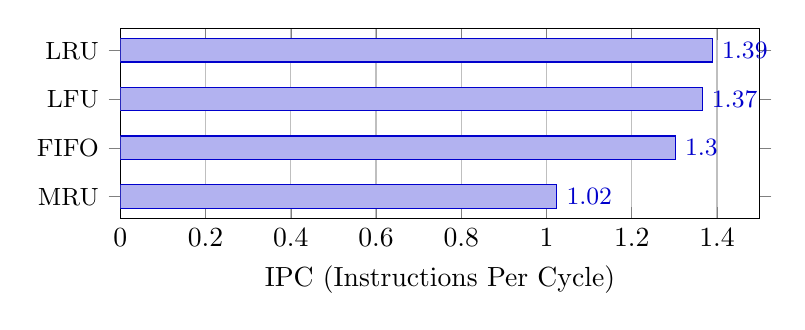
\begin{tikzpicture}
\begin{axis}[
    xbar,
    xmin=0,
    xmax=1.5,
    xlabel={IPC (Instructions Per Cycle)},
    ytick={1,2,3,4},
    yticklabels={LRU, LFU, FIFO, MRU}, % Modified order here
    yticklabel style={font=\small, text height=1.5ex},
    nodes near coords,
    nodes near coords style={font=\small},
    width=0.8\textwidth,
    height=4cm,
    bar width=0.3cm,
    xmajorgrids=true,
    enlarge y limits=0.15,
    y dir=reverse, % This flips the order to match your request
]
\addplot coordinates {
    (1.389,1) % LRU (now top)
    (1.365,2) % LFU 
    (1.302,3) % FIFO (moved up)
    (1.024,4) % MRU (now bottom)
};
\end{axis}
\end{tikzpicture}
\label{fig:ipc_hbars}
\end{figure}
\end{latin}

مقایسهٔ پارامتر Rate Hit

\begin{latin}
\begin{figure}[h]
\centering
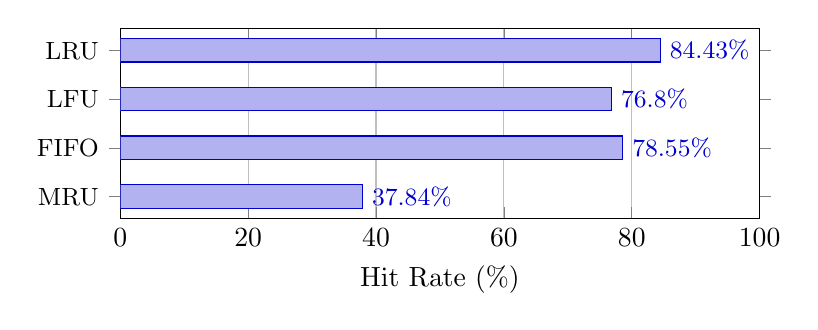
\begin{tikzpicture}
\begin{axis}[
    xbar,
    xmin=0,
    xmax=100,
    xlabel={Hit Rate (\%)},
    ytick={1,2,3,4},
    yticklabels={LRU, LFU, FIFO, MRU},
    yticklabel style={font=\small, text height=1.5ex},
    nodes near coords={\pgfmathprintnumber[fixed,precision=2]{\pgfplotspointmeta}\%},
    nodes near coords style={font=\small},
    width=0.8\textwidth,
    height=4cm,
    bar width=0.3cm,
    xmajorgrids=true,
    enlarge y limits=0.15,
    y dir=reverse,
    bar shift=0pt,
]
\addplot coordinates {
    (84.43,1) % LRU (top)
    (76.8,2)  % LFU
    (78.55,3) % FIFO
    (37.84,4) % MRU (bottom)
};
\end{axis}
\end{tikzpicture}
\label{fig:hitrate_bars}
\end{figure}
\end{latin}
می توان علت اصلی کارایی مطلوب LRU را به این دلیل دانست که از اصول Spatial Locality و Temporal Locality به خوبی بهره می گیرد و در عین حال پیچیدگی زیادی ندارد. البته شایان ذکر است که روش هایی مانند شبه LRU وجود دارند که پیچیدگی کمتری دارد. می توان ضعف LFU را در پیچیده بودن آن دانست. MRU هرچند ممکن است برای چینش های خاصی از Instruction ها مناسب باشد اما همان طور که در این شبیه سازی ها دیدیم، بدترین کارایی مربوط به MRU می شود.

\section{بخش امتیازی: پیاده سازی سیاست به وسیلهٔ پیش بینی تایم باقی مانده تا اخراج هر بلاک Mockingjay}

در این سیاست سه جزء اساسی وجود دارد: 
\begin{latin}
\begin{itemize}
	\item Sampled Cache
	\item RDP = Reuse Distance Predictor
	\item ETR = Estimate Time Remaining
\end{itemize}	
\end{latin}

روند کلی به این صورت است که ابتدا یک مجموعه از ست ها را که به صورت عادلانه در LLC پخش شده اند را انتخاب کرده و به عنوان سمپل های خود در نظر می گیریم و در Cache Sampled قرار می دهیم. در این ساختمان داده همچنین آخرین کلاکی که در آن درخواست دسترسی به آن بلاک را دریافت کردیم و نیز به همراه سایر اطلاعات مورد نیاز که در ادامه آن ها را شرح خواهیم داد در ساختمان داده ذخیره می کنیم.

پس از این با گرفتن هر Hit جدید فاصلهٔ بین کلاک قبلی که بلاک را دیده ایم تا الان محاسبه می کنیم و نتیجه را به همراه آدرس بلاک در اختیار RDP قرار می دهیم.

حال ماژول RDP وظیفه دارد تا با اطلاعاتی که از قبل پیش بینی کرده و فاصلهٔ جدیدی که دریافت کرده، پیش بینی قبلی اش را مورد ارزیابی قرار دهد.

برای این کار باید به outlier ها توجه کنیم تا پیش بینی ما دچار خطای زیادی نشود و مقدار تغییرات را حساب شده در پیش بینی خود تاثیر دهیم.

در نهایت هر گاه بلاک جدیدی وارد کش می شود مقدار اولیهٔ ETR خود را از RDP دریافت کرده و در هر کلاک از تمامی ETR های داخل کش یک واحد کم می شود. در نهایت در موقع اخراج بلاکی باید اخراج شود که بیشترین مقدار قدر مطلقی را دارد. چرا که هر چه این مقدار بیشتر باشد یعنی تا فراخوانی مجدد آن بلاک فاصلهٔ بیشتری داریم.

همچنین شایان ذکر است اگر با دو مقدار مساوی ماکزیمم مواجه شدیم و مقدار اصلی آنها یکی منفی و دیگری مثبت بود، باید آنی را که منفی است اخراج کنیم چرا که در واقع overdue شده است.

حال با جزئیات به این سه ماژول و پیاده سازی آن ها می پردازیم:

\subsection{\lr{Sampled Cache}}
ابتدا باید مشخص کنیم که چه ست هایی را قرار است به عنوان نمونه یاد بگیریم. در مجموع فرض کنید قرار است ۳۲ نمونه ست را یاد بگیریم.
پس بهتر است ست های ۰ و ۳۲ و ۶۴ و ... را انتخاب کنیم.

پس از این باید ببینیم ست فراخوانی شدهٔ جدید آیا در لیست سمپل های ما قرار دارد یا خیر. اگر قرار ندارد که کاری نیاز نداریم انجام بدهیم.

اما اگر قرار داشته باشد، باید حال در همین کش sample شدهٔ خودمان آیا از پیش قرار داشته یا خیر.

اگر از پیش قرار داشته، کافی است فاصله اش را از فرمول زیر حساب کرده:

\begin{center}
\begin{latin}
\text{reused distance} = \text{current time} - \text{last time}	
\end{latin}
\end{center}

و سپس این فاصله را در اختیار RDP گذاشته تا بر اساس آن پیش بینی اش را دقیق تر نماید. در ادامه باید time last و شمارهٔ PC این entry را آپدیت کنیم.

حال اگر از قبل در کش Sampled این entry وجود نداشت یعنی با miss مواجه هستیم و حالا باید یکی از مقادیر موجود در کش را اخراج کنیم. در این مرحله از همان سیاست LRU استفاده کرده و قربانی را اخراج می کنیم. باید این را ذکر کنیم که این قربانی را می توان SCAN دانست یعنی تنها یک بار مورد استفاده قرار گرفته و در ادامه دیگر به آن دسترسی انجام نشده به همین دلیل فاصلهٔ آن را $\infty $قرار می دهیم.

می توان این توضیحات فارسی را به شکل یک الگوریتم این گونه نشان داد:

\begin{latin}
\begin{algorithm}
\caption{Sample Cache}\label{alg:sca}
\begin{algorithmic}[1]
\Require Memory address, Program Counter (PC)
\Statex
\Function{SCA}{address, PC}
    \State $\text{set\_index} \gets (\text{address} \div \text{\# of blocks}) \bmod \text{\# of sets}$
    \State $x \gets \text{total number of sets}$
    \State $y \gets \text{number of samples}$
    \State $\text{sampleList} \gets [0, \dfrac{x}{y}, 2\dfrac{x}{y}, 3\dfrac{x}{y}, 4\dfrac{x}{y}, \dots] \quad \text{[5 ways]}$
    \Statex
    \If{$\text{set\_index} \in \text{sampleList}$}
        \State $\text{tag} \gets \text{setTag}(\text{address})$
        \State $\text{entry} \gets \text{SampleCache.Find}(\text{set\_index}, \text{tag})$
        \If{entry}
            \State $\text{lastTime} \gets \text{entry\_timestamp}$
            \State $\text{PC} \gets \text{entry.PC}$
            \State $\text{reused\_distance} \gets \text{currentTime} - \text{lastTime}$
            \State $\text{RDP\_train}(\text{PC}, \text{reused\_distance})$
            \State $\text{entry\_timestamp} \gets \text{current\_time}$
            \State $\text{entry.PC} \gets \text{PC}$
        \Else
            \State $\text{victim} \gets \text{SampleCache.Find\_victim}(\text{set\_index})$
            \State $\text{victim\_PC} \gets \text{victim.PC}$
            \State $\text{RDP\_train}(\text{victim\_PC}, \infty)$ \Comment{This is a scan}
            \State $\text{victim\_valid\_bit} \gets 1$
            \State $\text{victim\_tag} \gets \text{tag}$
            \State $\text{victim.PC} \gets \text{PC}$
            \State $\text{victim\_last\_Time} \gets \text{current\_Time}$
        \EndIf
    \EndIf
\EndFunction
\end{algorithmic}
\end{algorithm}
\end{latin}

\newpage
حال بر اساس همین الگوریتم که بر آمده از مقالهٔ معرفی شده است، کد C را می توانیم این گونه بازنویسی کنیم:

\begin{LTR}
\begin{lstlisting}
for (int i = 0; i < 32; ++i) {
        sampled_set_indices.push_back(i * (NUM_SET / 32));
    }
\end{lstlisting}
\end{LTR}
    
\begin{LTR}
\begin{lstlisting}
void SampledCache::handle_access(uint64_t full_addr, uint64_t pc_signature, int set_in_llc, int current_timestamp) {
    uint32_t internal_set = set_in_llc % NUM_SETS;
    uint64_t tag = full_addr >> 12;

    int hit_way = -1;
    for (int i = 0; i < NUM_WAYS; ++i) {
        if (sets[internal_set][i].valid && sets[internal_set][i].tag == tag) {
            hit_way = i;
            break;
        }
    }

    if (hit_way != -1) {
        auto& entry = sets[internal_set][hit_way];
        int time_elapsed = (current_timestamp >= entry.timestamp) ? (current_timestamp - entry.timestamp) : (current_timestamp - entry.timestamp + 256);
        
        rdp.train(entry.pc_signature, time_elapsed);

        entry.pc_signature = pc_signature;
        entry.timestamp = current_timestamp;
    } else {
        int victim_way = -1;
        int max_age = -1;
        for (int i = 0; i < NUM_WAYS; ++i) {
            if (!sets[internal_set][i].valid) {
                victim_way = i;
                break;
            }
            int age = (current_timestamp >= sets[internal_set][i].timestamp) ? (current_timestamp - sets[internal_set][i].timestamp) : (current_timestamp - sets[internal_set][i].timestamp + 256);
            if (age > max_age) {
                max_age = age;
                victim_way = i;
            }
        }
        
        if (sets[internal_set][victim_way].valid) {
            rdp.train(sets[internal_set][victim_way].pc_signature, RDP::INF_RD);
        }

        sets[internal_set][victim_way] = {true, tag, pc_signature, current_timestamp};
    }
}
\end{lstlisting}
\end{LTR}

\subsection{\lr{RDP}}
حال به سراغ RDP می رویم که شامل دو بخش است. predict و train

تابع predict صرفا با استفاده از بیت های پایینی PC مقادیر پیش بینی شده را بر می گرداند.

اما دربارهٔ train همان طور که گفته شد بر اساس اختلاف فاصلهٔ دو درخواست از یک entry یکسان عمل می کند و زمان درخواست بعدی را با الگوریتم سادهٔ زیر پیش بینی می کند:

\begin{latin}
\begin{algorithm}
\caption{RDP Train Algorithm}\label{alg:rdp_train}
\begin{algorithmic}[1]
\Require Program Counter (PC), observed distance
\Statex
\Function{RDP\_Train}{PC, observed\_distance}
    \State $\text{entry} \gets \text{RDP.Find}(\text{PC})$
    \State $\text{old\_Prediction} \gets \text{entry.predicted\_distance}$
    \State $\text{diff} \gets \text{observed\_distance} - \text{old\_Prediction}$
    \State $\text{nudge} \gets \min\left(1, \frac{|\text{diff}|}{16}\right)$
    \Statex
    \If{$\text{observed\_distance} > \text{old\_prediction}$}
        \State $\text{entry.predicted\_distance} \gets \text{entry.predicted\_distance} + \text{nudge}$
    \Else
        \State $\text{entry.predicted\_distance} \gets \text{entry.predicted\_distance} - \text{nudge}$
    \EndIf
\EndFunction
\end{algorithmic}
\end{algorithm}
\end{latin}

حال به راحتی می توان این شبه کد را به زبان C تبدیل کرد:
\begin{LTR}
\begin{lstlisting}
int RDP::temporal_difference(int init, int sample) {
    if (sample > init) {
        int diff = (sample - init) / 16;
        return min(init + max(1, diff), INF_RD);
    }
    if (sample < init) {
        int diff = (init - sample) / 16;
        return max(init - max(1, diff), 0);
    }
    return init;
}
\end{lstlisting}
\end{LTR}

\begin{LTR}
\begin{lstlisting}
void RDP::train(uint64_t pc_signature, int sample) {
    uint32_t index = pc_signature % PREDICTOR_SIZE;
    rdp_table[index] = temporal_difference(rdp_table[index], sample);
}
\end{lstlisting}
\end{LTR}

\subsection{ETR}
با توجه به توضیحات داده شده به راحتی می توان الگوریتم این بخش را نیز به شکل زیر نوشت:

\begin{latin}
\begin{algorithm}
\caption{ETR-Based Victim Selection}\label{alg:etr_victim}
\begin{algorithmic}[1]
\Require triggering\_cpu, instr\_id, set, current\_set, ip, full\_addr, type
\Ensure Victim way index or NUM\_WAY if no victim found
\Statex
\Function{find\_victim}{triggering\_cpu, instr\_id, set, current\_set, ip, full\_addr, type}
    \For{$i \gets 0$ \textbf{to} $\text{NUM\_WAY} - 1$}
        \If{$\text{current\_set}[i].\text{valid} = \text{false}$}
            \State \Return $i$ \Comment{Return first invalid way}
        \EndIf
    \EndFor
    \Statex
    \State $\text{pc\_signature} \gets \text{get\_pc\_signature}(\text{ip}, \text{false})$
    \State $\text{predicted\_rd} \gets \text{rdp.predict}(\text{pc\_signature})$
    \If{$\text{type} \neq \text{WRITE} \land (\text{predicted\_rd} > \text{MAX\_RD\_THRESHOLD})$}
        \State \Return $\text{NUM\_WAY}$ \Comment{No victim found case}
    \EndIf
    \Statex
    \State $\text{victim\_way} \gets 0$
    \State $\text{max\_abs\_etr} \gets -1$
    \For{$i \gets 0$ \textbf{to} $\text{NUM\_WAY} - 1$}
        \State $\text{current\_etr} \gets \text{etr\_counters}[\text{set}][i]$
        \State $\text{current\_abs\_etr} \gets |\text{current\_etr}|$
        \Statex
        \If{$\text{current\_abs\_etr} > \text{max\_abs\_etr}$}
            \State $\text{max\_abs\_etr} \gets \text{current\_abs\_etr}$
            \State $\text{victim\_way} \gets i$
        \ElsIf{$\text{current\_abs\_etr} = \text{max\_abs\_etr}$}
            \If{$\text{etr\_counters}[\text{set}][\text{victim\_way}] \geq 0 \land \text{current\_etr} < 0$}
                \State $\text{victim\_way} \gets i$ \Comment{Prefer negative ETR when tied}
            \EndIf
        \EndIf
    \EndFor
    \State \Return $\text{victim\_way}$
\EndFunction
\end{algorithmic}
\end{algorithm}
\end{latin}
\newpage
و کد C متناظر به این شکل است:
\begin{LTR}
\begin{lstlisting}
long myMOCKINGJAY::find_victim(...) {
    for (long i = 0; i < NUM_WAY; ++i) {
        if (!current_set[i].valid) {
            return i;
        }
    }

    uint64_t pc_signature = get_pc_signature(ip.to<uint64_t>(), false);
    int predicted_rd = rdp.predict(pc_signature);
    if (type != access_type::WRITE && (predicted_rd > MAX_RD_THRESHOLD)) {
        return NUM_WAY;
    }

    long victim_way = 0;
    int max_abs_etr = -1;
    for (long i = 0; i < NUM_WAY; ++i) {
        int current_etr = etr_counters[set][i];
        int current_abs_etr = abs(current_etr);

        if (current_abs_etr > max_abs_etr) {
            max_abs_etr = current_abs_etr;
            victim_way = i;
        } else if (current_abs_etr == max_abs_etr) {
            if (etr_counters[set][victim_way] >= 0 && current_etr < 0) {
                victim_way = i;
            }
        }
    }
    return victim_way;
}
\end{lstlisting}
\end{LTR}

در آخر نیز باید اشاره کنیم با هر hit باید یک عدد از ETR ها کم شود به شرط آنکه آن entry یک SCAN نباشد. همچنین باید چک کنیم که آیا فراخوانی اخیر جزوی از sample های ما است یا خیر و اگر هست باید آن را در اختیار Cache Sampled نیز قرار بدهیم:

\begin{LTR}
\begin{lstlisting}
void myMOCKINGJAY::update_replacement_state(uint32_t triggering_cpu, long set, long way, champsim::address full_addr, champsim::address ip,
                                  champsim::address victim_addr, access_type type, uint8_t hit) {
    if (way >= NUM_WAY) return;
    if (type == access_type::WRITE) return;

    uint64_t pc_signature = get_pc_signature(ip.to<uint64_t>(), hit);

    if (hit) {
        int predicted_rd = rdp.predict(pc_signature);
        etr_counters[set][way] = (predicted_rd > MAX_RD_THRESHOLD) ? INF_ETR : predicted_rd / GRANULARITY;
    }

    etr_clock[set]++;
    if (etr_clock[set] >= GRANULARITY) {
        etr_clock[set] = 0;
        for (int i = 0; i < NUM_WAY; ++i) {
            if (abs(etr_counters[set][i]) < INF_ETR) {
                etr_counters[set][i]--;
            }
        }
    }
    
    if (is_sampled_set(set)) {
        set_timestamps[set] = (set_timestamps[set] + 1) % 256;
        sampled_cache.handle_access(full_addr.to<uint64_t>(), pc_signature, set, set_timestamps[set]);
    }
}
\end{lstlisting}
\end{LTR}

\subsection{مقایسهٔ عملکرد}
با مبنا قرار دادن همان دستور قبلی با ۶۰ میلیون دستور warmup و ۴۰ میلیون دستور شبیه سازی و با همان trace گذشته، مقادیر IPC و Rate Hit را مقایسه می کنیم:

\begin{latin}
\begin{figure}[h]
\centering
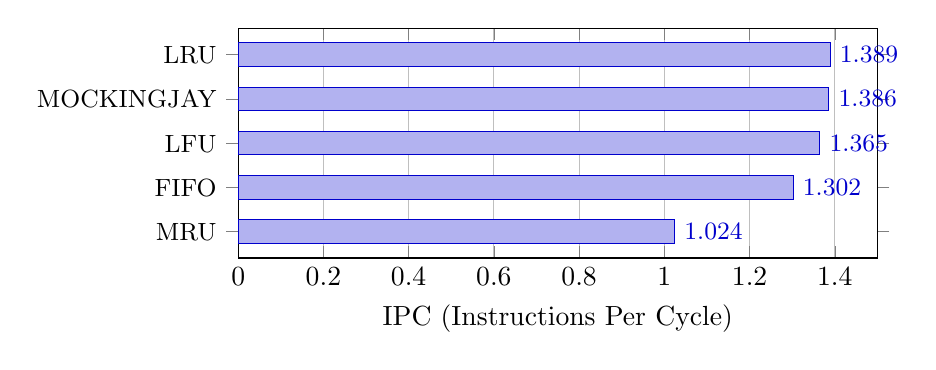
\begin{tikzpicture}
\begin{axis}[
    xbar,
    xmin=0,
    xmax=1.5,
    xlabel={IPC (Instructions Per Cycle)},
    ytick={1,2,3,4,5},
    yticklabels={LRU, MOCKINGJAY, LFU, FIFO, MRU}, % Reordered labels
    yticklabel style={font=\small, text height=1.5ex},
    nodes near coords={\pgfmathprintnumber[precision=3]{\pgfplotspointmeta}},
    nodes near coords style={font=\small},
    width=0.8\textwidth,
    height=4.5cm,
    bar width=0.3cm,
    xmajorgrids=true,
    enlarge y limits=0.15,
    y dir=reverse,
]
\addplot coordinates {
    (1.389,1) % LRU (top)
    (1.386,2) % MOCKINGJAY (new position)
    (1.365,3) % LFU 
    (1.302,4) % FIFO
    (1.024,5) % MRU (bottom)
};
\end{axis}
\end{tikzpicture}
\label{fig:ipc_hbars}
\end{figure}
\end{latin}

\begin{latin}
\begin{figure}[h]
\centering
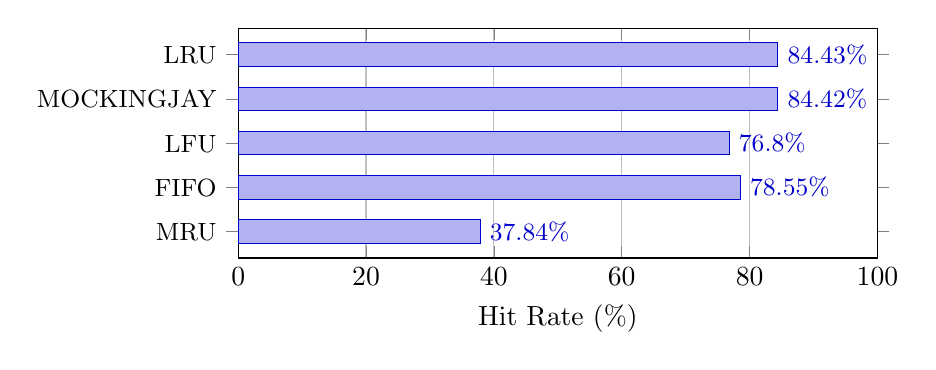
\begin{tikzpicture}
\begin{axis}[
    xbar,
    xmin=0,
    xmax=100,
    xlabel={Hit Rate (\%)},
    ytick={1,2,3,4,5},
    yticklabels={LRU, MOCKINGJAY, LFU, FIFO, MRU}, % MOCKINGJAY inserted
    yticklabel style={font=\small, text height=1.5ex},
    nodes near coords={\pgfmathprintnumber[fixed,precision=2]{\pgfplotspointmeta}\%}, % Force 2 decimal places
    nodes near coords style={font=\small},
    width=0.8\textwidth,
    height=4.5cm, % Slightly taller to fit 5 bars
    bar width=0.3cm,
    xmajorgrids=true,
    enlarge y limits=0.15,
    y dir=reverse,
    bar shift=0pt,
]
\addplot coordinates {
    (84.43,1)  % LRU (top)
    (84.42,2)  % MOCKINGJAY (new entry)
    (76.80,3)  % LFU (now 76.80 for consistency)
    (78.55,4)  % FIFO
    (37.84,5)  % MRU (bottom)
};
\end{axis}
\end{tikzpicture}
\label{fig:hitrate_bars}
\end{figure}
\end{latin}

اما خالی از لطف نیست تا این سیاست ها را روی یک trace دیگر مانند lbm\_104B که ساختار پیچیده ای دارد نیز انجام دهیم:

\begin{latin}
\begin{figure}[h]
\centering
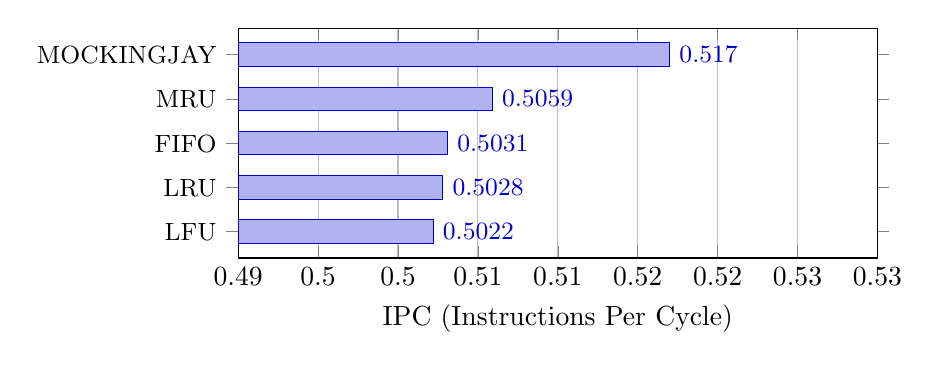
\begin{tikzpicture}
\begin{axis}[
    xbar,
    xmin=0.49,
    xmax=0.53,
    xlabel={IPC (Instructions Per Cycle)},
    ytick={1,2,3,4,5},
    yticklabels={MOCKINGJAY, MRU, FIFO, LRU, LFU}, % Sorted high to low
    yticklabel style={font=\small, text height=1.5ex},
    nodes near coords={\pgfmathprintnumber[fixed,precision=4]{\pgfplotspointmeta}}, % 4 decimal places
    nodes near coords align={horizontal},
    nodes near coords style={font=\small},
    width=0.8\textwidth,
    height=4.5cm,
    bar width=0.3cm,
    xmajorgrids=true,
    enlarge y limits=0.15,
    y dir=reverse,
]
\addplot coordinates {
    (0.5170,1)  % MOCKINGJAY (highest)
    (0.5059,2)  % MRU
    (0.5031,3)  % FIFO
    (0.5028,4)  % LRU
    (0.5022,5)  % LFU (lowest)
};
\end{axis}
\end{tikzpicture}
\label{fig:ipc_bars}
\end{figure}
\end{latin}

در کل می توان گفت در توزیع های مختلف داده عملکرد مشابهی با LRU داشته اما زمانی که الگوی موجود در داده پیچیده باشد مانند ،lbm عملکرد بهتری در مقایسه با دیگر سیاست ها نشان می دهد.

از دیدگاه پیچیدگی می توان گفت در میان این ۵ سیاست، از همه پیچیدگی بیشتری داشته و حافظهٔ بیشتری نسبت به آنها اشغال می کند. چرا که دارای ۳ بخش است که هر یک باید داده هایی را ذخیره کنند.

اما با این حال به دلیل آن که پیش بینی زمان انجام فراخوانی ها بسیار کمک کننده است، نسبت به سایر سیاست ها کارایی نامطلوبی نداشته و در تست های مختلف با توزیع داده های گوناگون کارایی مناسبی دارد.


\end{document}